% ncse_new/p1_SystemsOfEquations/ch1_MatVec/ex_ArrowMatrixVector.tex
% the exercise requires:    arrowmatvec.m    arrowmatvectiming.eps    arrowmatvectiming.jpg
% the solutions require:    arrowmatvec2.m    arrowmatvec2timing.m    arrowmatvec2timing.eps

\renewcommand{\chpt}{ch_matvec}

\begin{problem}[Arrow matrix-vector multiplication \coreproblem] \label{prb:ArrowMatrixVector}

Consider the multiplication of the two ``arrow matrices'' $\VA$ with a vector $\Vx$,
implemented as a function \texttt{arrowmatvec(d,a,x)} in the following \Matlab~ script
%
\lstinputlisting[caption={multiplying a vector with the product of two ``arrow matrices''},label={mc:ArrowMatrixVector_arrowmatvec}]
{\problems/\chpt/MATLAB/arrowmatvec.m}
%

%%%%%%%%%%%% SUBPROBLEM 1

\begin{subproblem}[1] \label{subprb:ArrowMatrixVector_1}
For general vectors $d = (d_1, \dots, d_n)^\top$ and $a = (a_1, \dots, a_n)^\top$, sketch the matrix $\VA$  created in line 6 of \autoref{mc:ArrowMatrixVector_arrowmatvec}.

\begin{hint}
This \Matlab~ script is provided as file \texttt{arrowmatvec.m}.
\end{hint}

\begin{solution}
$\VA=\begin{pmatrix}
         d_1 &     &        &         &  a_1     \\
             & d_2 &        &         &  a_2     \\
             &     & \ddots &         &  \vdots  \\
             &     &        & d_{n-1} &  a_{n-1} \\
         a_1 & a_2 & \dots  & a_{n-1} &  d_n     \\
 \end{pmatrix}$
\end{solution}
\end{subproblem}

%%%%%%%%%%%% SUBPROBLEM 2

\begin{subproblem}[2] \label{subprb:ArrowMatrixVector_2}
The \texttt{tic-toc} timing results for \texttt{arrowmatvec.m} are available in
\autoref{fig:arrowmatvectiming}.  Give a detailed explanation of the results.

\begin{figure}[ht]
\centering
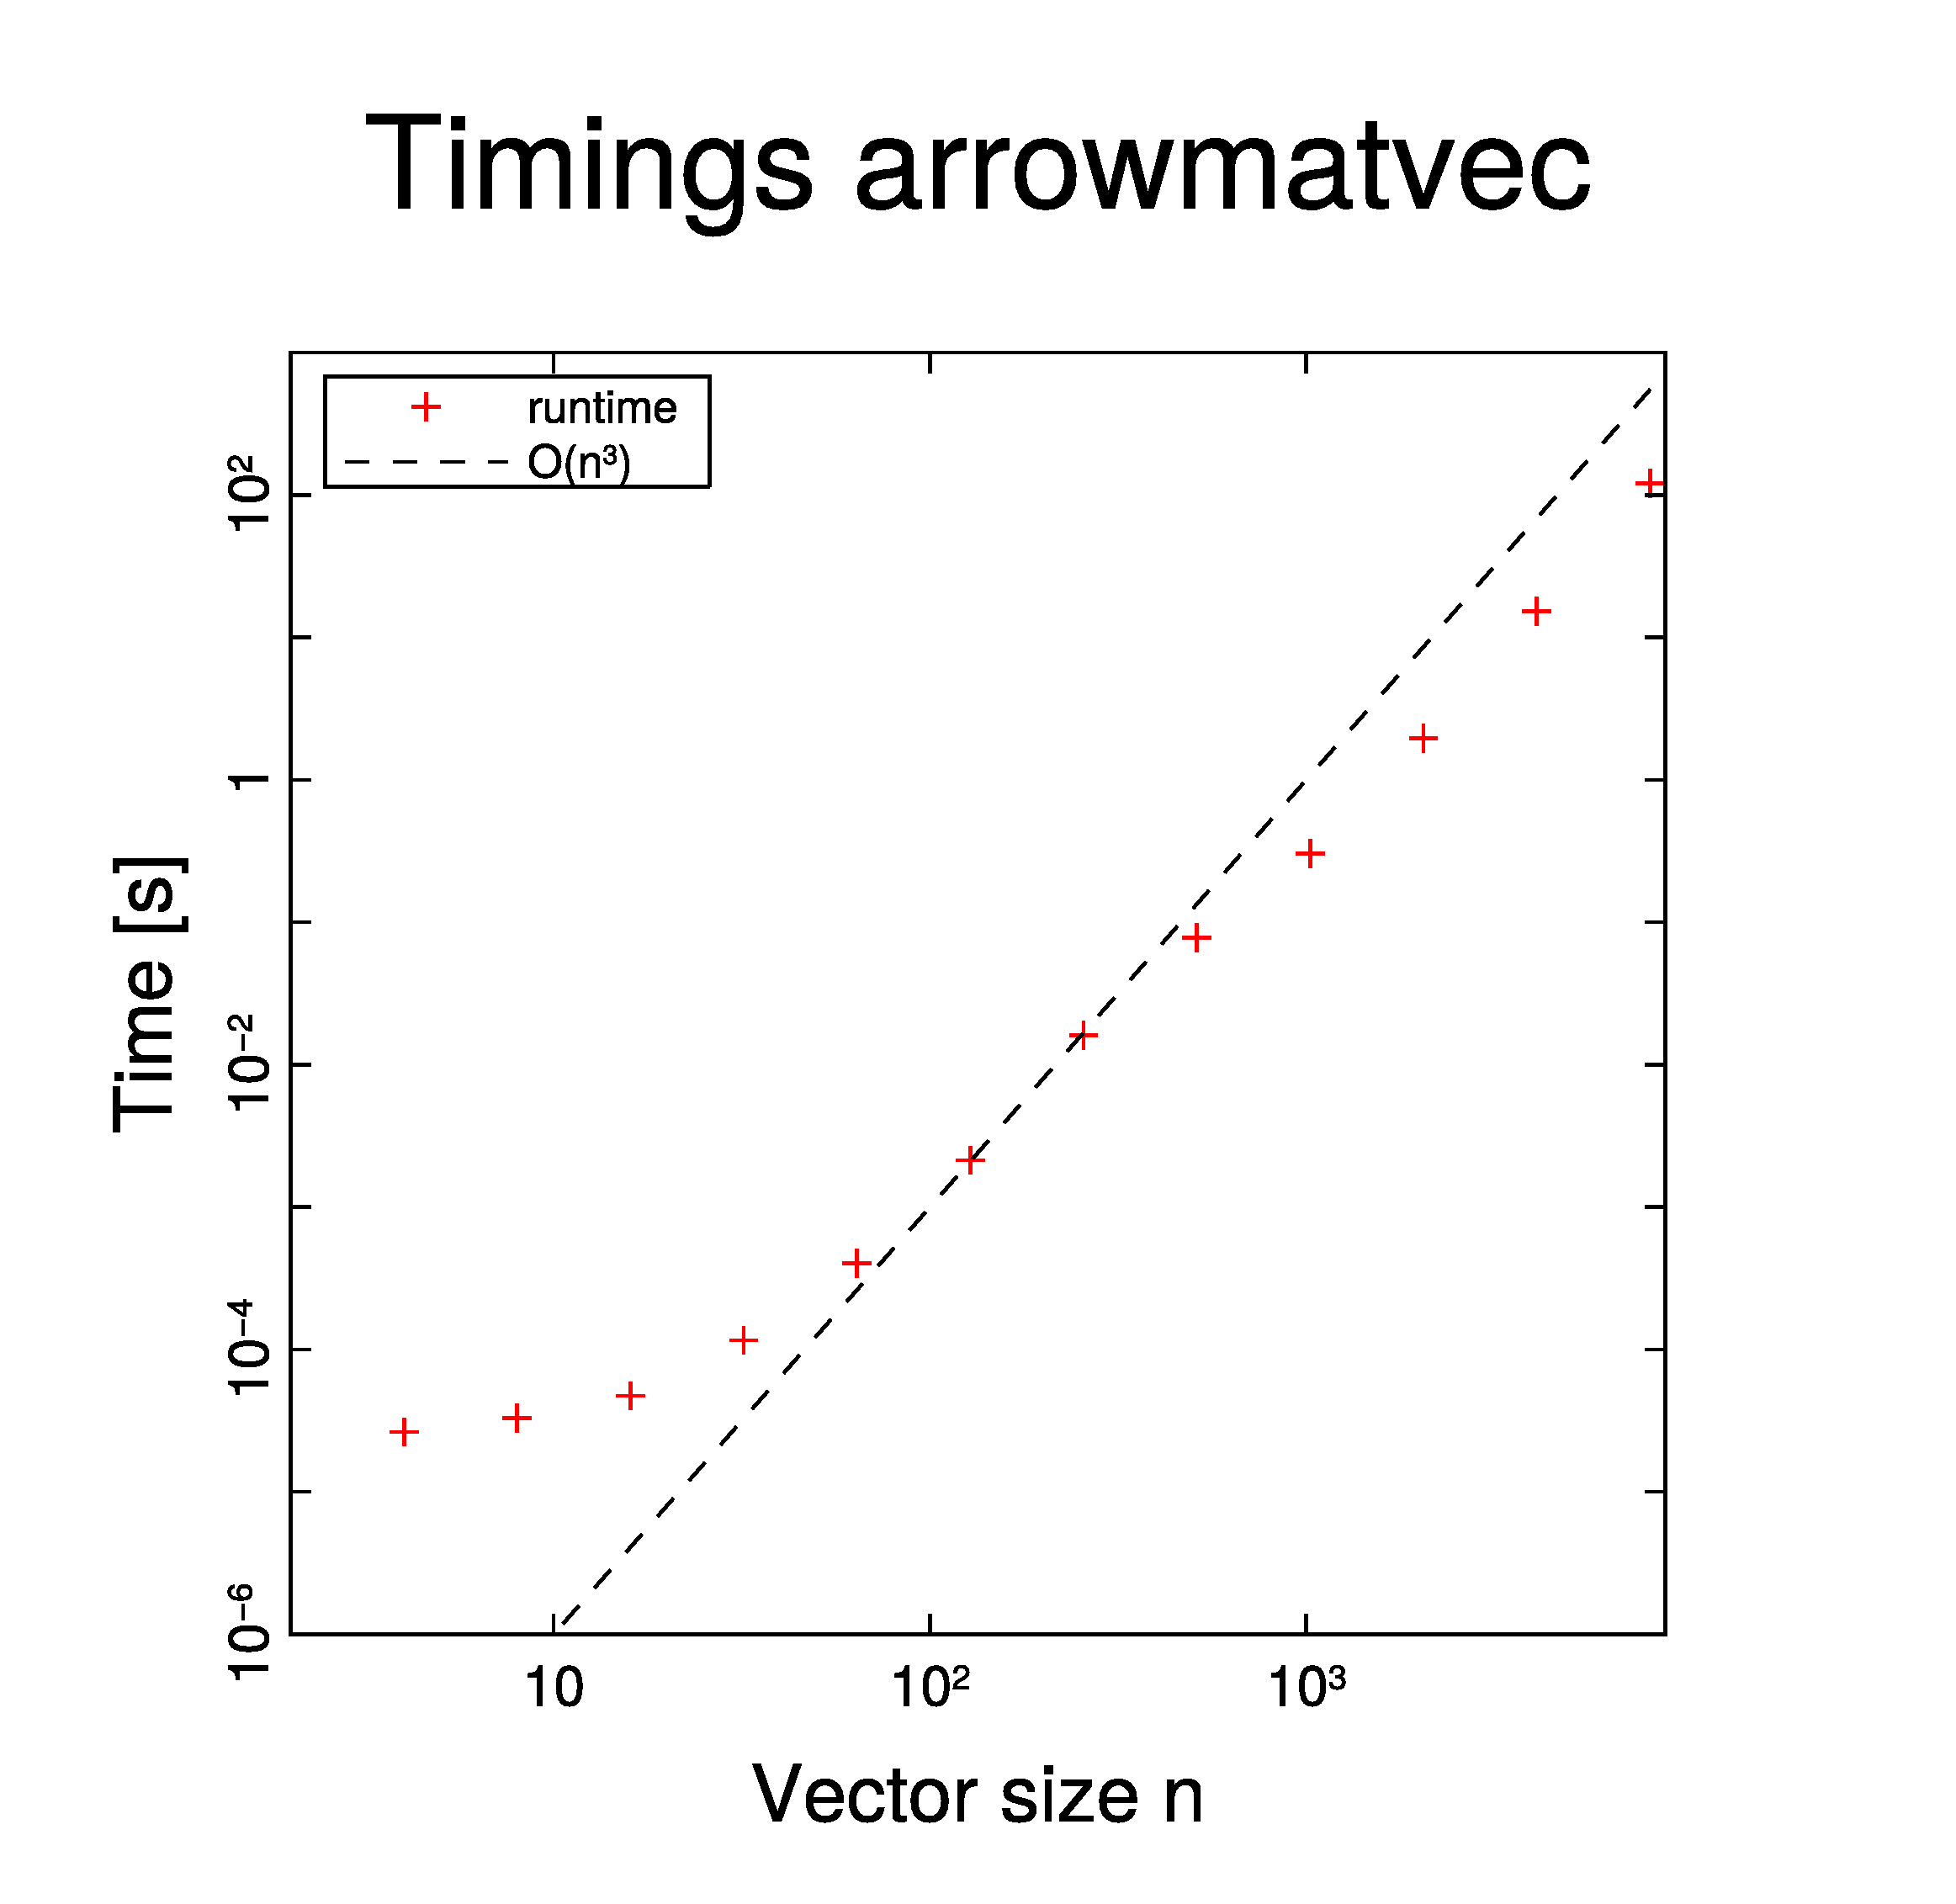
\includegraphics[width=0.8\textwidth]{\problems/\chpt/PICTURES/arrowmatvectiming.eps}
\caption{timings for \texttt{arrowmatvec(d,a,x)}}
\label{fig:arrowmatvectiming}
\end{figure}


\begin{hint}
This \Matlab~ created figure is provided as file
\texttt{arrowmatvectiming.\{eps,jpg\}}.
\end{hint}

\begin{solution}
The standard matrix-matrix multiplication has runtimes growing with $O(n^3)$ and the standard matrix-vector multiplication has runtimes growing with $O(n^2)$. Hence, the overall computational complexity is dominated by $O(n^3)$.
\end{solution}
\end{subproblem}

%%%%%%%%%%%% SUBPROBLEM 3

\begin{subproblem}[3]  \label{subprb:ArrowMatrixVector_3}
Write an \emph{efficient} \Matlab~ function 
\begin{center}
  \texttt{function y = arrowmatvec2(d,a,x)}
\end{center}
that computes the same multiplication as in code \ref{mc:ArrowMatrixVector_arrowmatvec} but with optimal asymptotic complexity with respect to {$n$}.
Here \texttt{d} passes the vector $(d_{1},\ldots,d_{n})^{T}$ and \texttt{a} passes the vector $(a_{1},\ldots,a_{n})^{T}$.

\begin{solution}
 Due to the sparsity and special structure of the matrix, it is possible to write a more efficient implementation than the standard matrix-vector multiplication. See code listing \ref{mc:ArrowMatrixVector_arrowmatvec2}
\vspace{0.5cm}

\lstinputlisting[caption={implementation of the function \texttt{arrowmatvec2}},label={mc:ArrowMatrixVector_arrowmatvec2}]
{\problems/\chpt/MATLAB/arrowmatvec2.m}
\end{solution}
\end{subproblem}

%%%%%%%%%%%% SUBPROBLEM 4

\begin{subproblem}[1]  \label{subprb:ArrowMatrixVector_4}
What is the complexity of your algorithm from sub-problem
\ref{subprb:ArrowMatrixVector_3} (with respect to problem size $n$)? 

\begin{solution}
The efficient implementation only needs two vector-vector element-wise multiplications and one vector-scalar multiplication. Therefore the complexity is $O(n)$.
\end{solution}
\end{subproblem}

%%%%%%%%%%%% SUBPROBLEM 5

\begin{subproblem}[2] \label{subprb:ArrowMatrixVector_5}
Compare the runtime of your implementation and the implementation given in code \ref{mc:ArrowMatrixVector_arrowmatvec} for $n=2^{5,6,\ldots,12}$.
Use the routines \texttt{tic} and \texttt{toc} as explained in example \ncseex{ex:effmatmult} of the Lecture Slides.

\begin{solution}
The standard matrix multiplication has runtimes growing with $O(n^3)$.
The runtimes of the more efficient implementation are growing with $O(n)$.
See \autoref{mc:ArrowMatrixVector_arrowmatvec2timing} and Figure~\ref{fig:arrowmatvec2timing}.

\lstinputlisting[caption={Execution and timings of \texttt{arrowmatvec} and \texttt{arrowmatvec2}}, label={mc:ArrowMatrixVector_arrowmatvec2timing}]
{\problems/\chpt/MATLAB/arrowmatvec2timing.m}

\begin{figure}[ht]
\centering
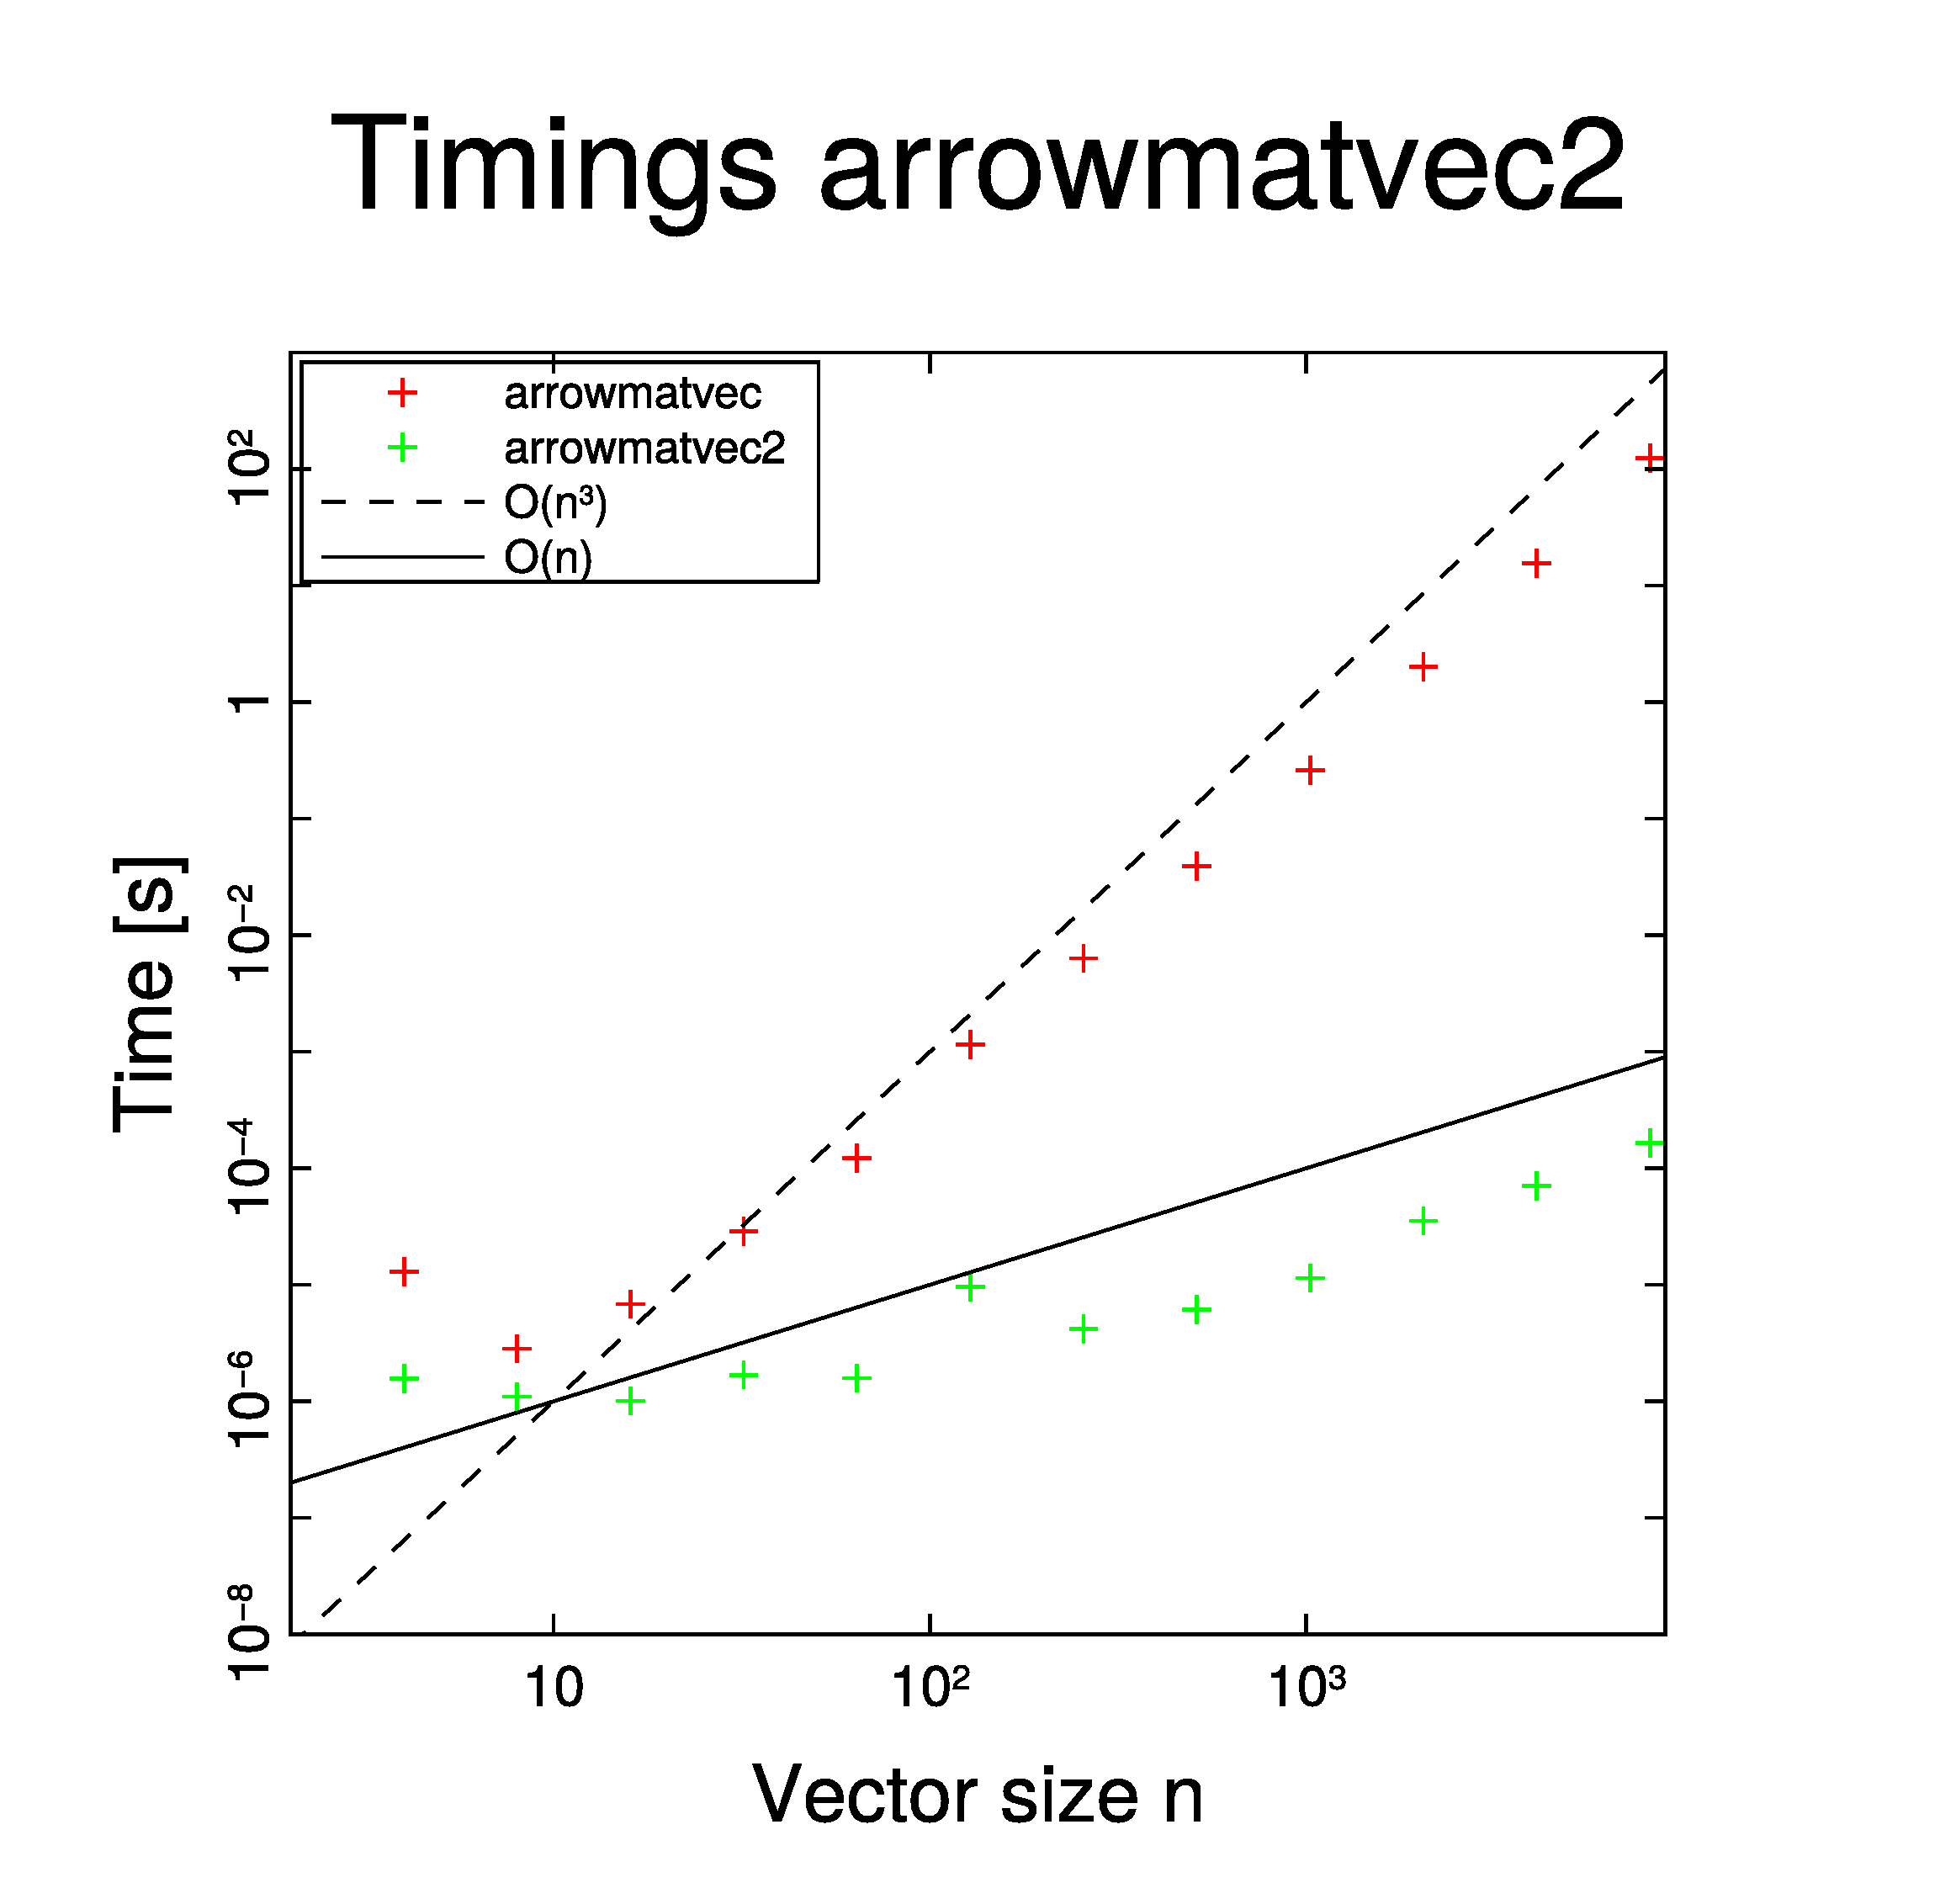
\includegraphics[width=0.8\textwidth]{\problems/\chpt/PICTURES/arrowmatvec2timing.eps}
\caption{timings for \texttt{arrowmatvec2(d,a,x)}} \label{fig:arrowmatvec2timing}
\end{figure}
\end{solution}
\end{subproblem}

\begin{subproblem}[1] \label{subprb:ArrowMatrixVector_6}
Write the \eigen{} codes corresponding to the functions \texttt{arrowmatvec} and \texttt{arrowmatvec2}.

\begin{solution}
See Listing~\ref{cppc:arrowmatvec} and Listing~\ref{cppc:arrowmatvec2}.

\lstinputlisting[style=cpp,caption={Implementation of \texttt{arrowmatvec}  in \eigen{}},label={cppc:arrowmatvec}]
{\problems/\chpt/CPP/arrowmatvec.cpp}

\lstinputlisting[style=cpp,caption={Implementation of \texttt{arrowmatvec2}  in \eigen{}},label={cppc:arrowmatvec2}]
{\problems/\chpt/CPP/arrowmatvec2.cpp}
\end{solution}
\end{subproblem}

\end{problem}
